%%%%%%%%%%%%%%%%%%%%%%%%%%%%%%%%%%%%%%%%%%%%%%
\section{Beamline instrumentation}
\label{sec:beaminstruments}

The H4 beamline will be instrumented with a number of beamline monitors to provide information 
\fixme{should we add "and trigger capability" ?}
 about the beam profile, position, momentum, and particle identification. 
 %A number of proposals are being evaluated NP04.  --- can't say this in a TDR ---
 In this section, the baseline design for the beam monitors are presented. 

\subsection{Beam profile monitoring, particle tracking and momentum measurements}
Operation of the beam line requires at least one beam  monitor, able to provide the beam profile in two dimensions at the end of the beamline.   The beam monitor can also be exploited for data analysis, provided that it delivers data on an event-by-event basis. Another monitor, located immediately downstream of the last bending magnet, is added in the layout  in order to determine the particle  direction and position and match it with the reconstructed track in the LAr active volume.

%\subsection{Momentum measurements}
The uncertainty in momentum resolution of the beam can be reduced by measuring the momentum particle by particle with a set of three detectors placed one before and two after one of the bending magnets. On paper, momentum resolutions of the order of 1\% could be achieved with this system, however  multiple scattering can affect the measurement at low energies. 
\fixme{We are writing a TDR and need to describe the performance of the device that we will use; e.g. "on paper ..." is not ok for a TDR. }
Preliminary results in full simulation point to a resolution better than 2\%. The same devices which are used for beam monitoring can also be used for momentum measurement.
%
\paragraph{Fiber tracker}
The CERN Beam Instrumentation (BI) group offers to produce
\fixme{This is a TDR. We can no longer write about proposal. Instead we need to describe what we are planing to build. One possibility could be to describe the primary system and then describe a potential back-up/alternate.}
 beam monitors based on scintillating fibers, which have a polystyrene core surrounded by cladding. Fibers provide a light yield ~8000 photons/MeV deposited with fast rise and decay times of 1-3 ns. The baseline design foresees 1mm square fibers in two planes to provide X and Y coordinates. Fibers will be mirrored on one end to increase
light collection.  Every monitor consisting of two planes of 1~mm thick fibers adds 0.47\% $X_0$ to the material budget.
A fiber plane is made out of 192 fibers with no space between them will ensure a  192mm $\times$ 192mm covered area and fits in the beamline.
Light can be read either with MultiAnode PMTs or with SiPMs, depending on the application (see below about the possible use for Time of Flight).
\fixme{Need to decide on one and describe that one.}
These monitors are designed to work inside the vacuum chamber and can be mounted on special flanges, without need to break the vacuum.

\paragraph{Multiwire Proportional Chambers}
Fermilab has multi-wire proportional chambers (MWPCs) with X-Y sense plane
readout, approximately 128 mm x 128 mm, readily available that can also be used as beam profile monitors. 
Chambers add 0.002 nuclear collision lengths and 0.007 radiation lengths.
\fixme{Should use consistent notation, e.g. all \% or fractions }
 These chambers have a long history, so installation, integration and commissioning should be straightforward. They are operated in air, thus would require to divide the beamline vacuum into sections.


\subsection{Particle identification}
The H4 beamline is capable of delivering two types of beams: electron and hadron beams. While the electron beam is relatively pure, the hadron beam consists of a mixture of electron, pion, kaon, and proton. Therefore it is essential to have an efficient particle identification system to cleanly tag particle types on a particle by particle basis. To achieve this goal, a particle identification system based on a combination of threshold Cherenkov counters and Time-of-flight system is being considered for ProtoDUNEs. 
\fixme{Again, "is being considered" is not appropriate for a TDR}
Cherenkov counters can be placed in the last segment of the beam line, in between the last bending magnet and the cryostat. Space for a ToF system is available provided that the detectors are compact enough,
\fixme{quantify "compact enough"}
and would allow a flight path of 23~m.

\paragraph{Threshold Cherenkov counter}
The threshold Cherenkov counters have been used extensively in beamlines to discriminate particles. Figure~\ref{fig:ckv} shows one of the counters used in the CERN test beam area. It consists of a gas radiator that is contained in a long cylindrical tube, and a detection box in which the Cherenkov light is reflected by a 45$^\circ$ mirror and focused onto a photomultiplier tube. The diameter of the cylindrical tube is designed to allow the counter to pass through the standard CERN beam pipe of about 20cm. A variety of gasses (e.g. CO2, nitrogen, argon, Freon 12, air) are available at CERN to optimize particle identification. The CERN beam group plans to install at least one (possibly two) threshold Cherenkov counter in the H4 beamline. 
\fixme{Cannot be written as is; need to describe benefit of one vs two threshold Cherenkov counters; baseline is presumably one counter; so, describe one and then say that there mat=y be additional benefits (which ?) if a second one is added.}
Figure~\ref{fig:ckv_gases} shows the gas pressure threshold 
for the production of Cherenkov light for various particle types as a function of particle momentum for Freon 12 and CO$_2$ gases.
\begin{cdrfigure}[CERN threshold Cherenkov counter]{ckv}{CERN threshold Cherenkov counter}
  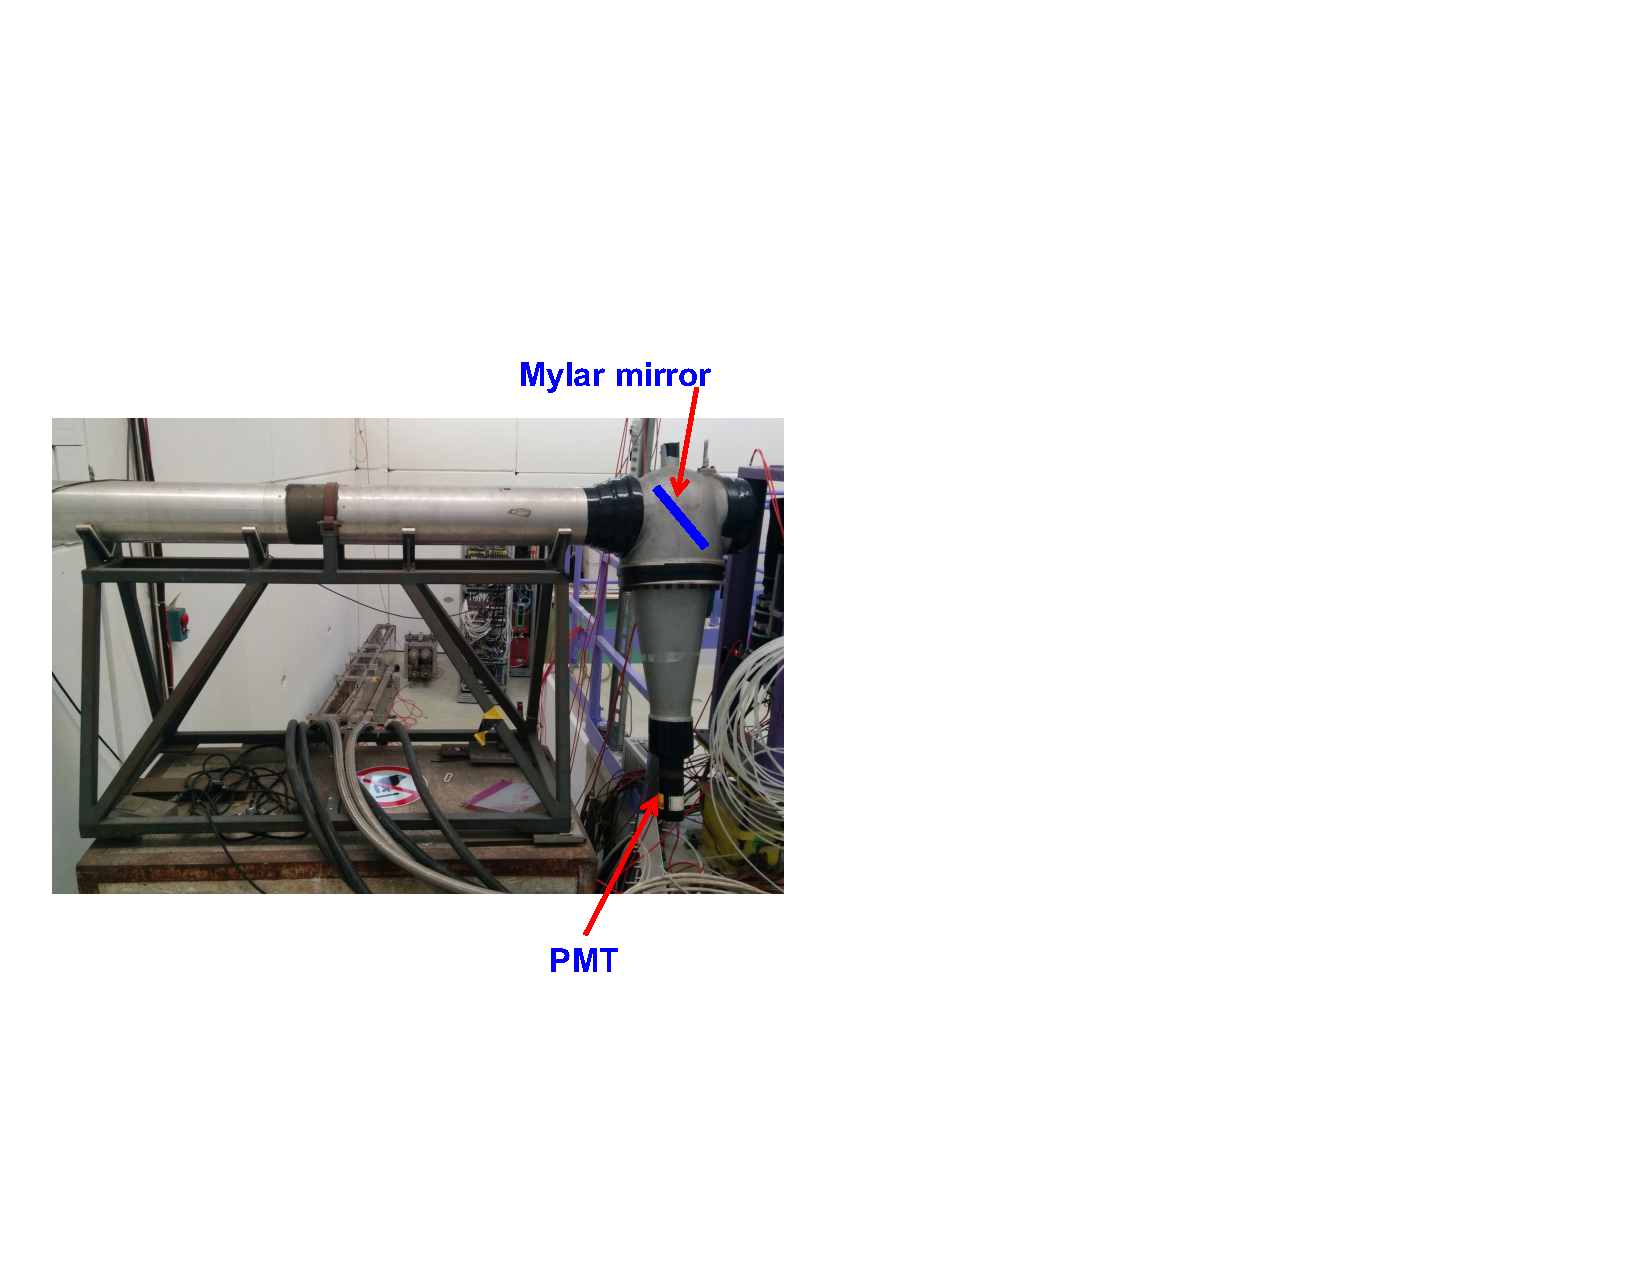
\includegraphics[width=0.65\textwidth]{beamline_ckv.pdf}
\end{cdrfigure}
\begin{cdrfigure}[Cherenkov gases]{ckv_gases}{Gas pressure threshold for the production of Cherenkov light for various particles as a function of particle momentum for Freon 12~\footnote{N. Charitonidis, Y. Karyotakis \it{et al.}, ``Hadron identification proposal for the ProtoDUNE experiments of CENF, to be published.} and CO$_2$ gases.}
  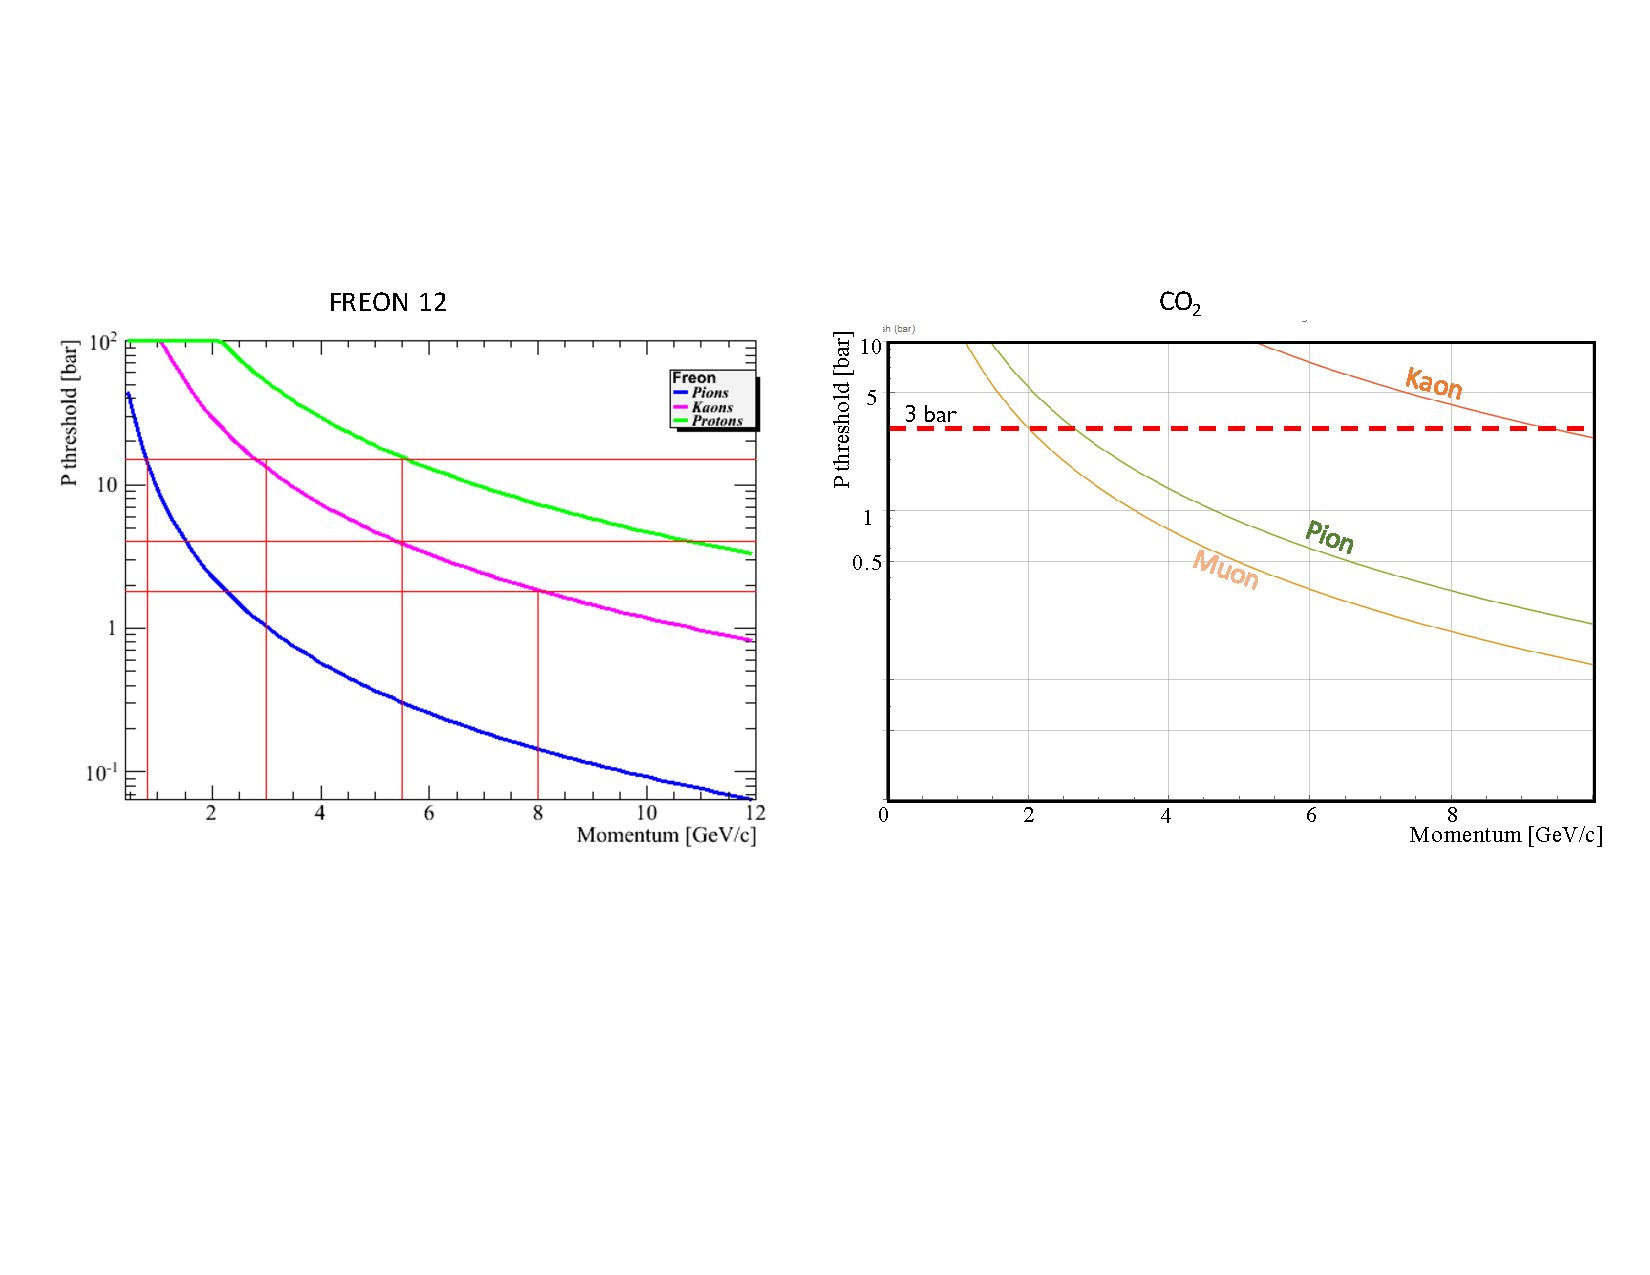
\includegraphics[width=0.99\textwidth]{beamline_CKVgases.pdf}
\end{cdrfigure}
Freon-12 has been selected for its high density, however it cannot be operated at pressures larger than 3bars to avoid liquefaction.  CO$_2$ can be used more easily at higher pressures.  Drawings for high pressure Cherenkov counters exist at CERN, thus a new one could be manufactured. 
\fixme{What is the plan ? Do we use an existing one or do we need to build one ?? This should be spelled out.}
 Figure~\ref{fig:ckv_gases} shows that pions can be tagged with a 3bars Freon counter for momenta larger that 2 GeV/c, and Kaons can be tagged with an high pressure  CO$_2$  counter above 4 GeV/c. 
At low energies, it will be essential  to tag electrons, that are the dominant component of the beam. This can be easily achieved with one   of the cherenkovs filled with CO$_2$ at low pressure.
\fixme{Above paragraph needs to be rewritten more clearly. As written it is confusing.}

A time-of-flight system  is therefore needed to distinguish hadrons below the mentioned thresholds.  From table \ref{tab:beampartcomp} it is evident that the Kaon content of the beam is negligible at least below 2 GeV/c, thus  only pion-proton separation is needed at low energies. Figure\ref{fig:toftau} shows the ToF resolution needed to distinguish among particle species at the $4\sigma$ level as a function of the particle momentum, assuming a 23~m long path. To distinguish pions from protons below 2 GeV/c a 1~ns resolution is enough, while 300ps are necessary for kaon-proton up to  4~GeV/c. It has also to be noted that a ToF system with a ~100ps resolution would allow to identify protons from other hadrons up to 7~GeV, so that the high pressure CO$_2$ Cherenkov could be avoided. Conversely, in order to cover all the energy range up to 7~GeV for all hadron  types, a ToF system with a resolution better than 40~ps would be needed.
In the following, two (possibly complementary) ToF systems are described.
\begin{cdrfigure}[Required ToF resolution]{toftau}{Required ToF resolution to  distinguish among particle species at the $4\sigma$ level as a function of the particle momentum, assuming a 23~m long path. }
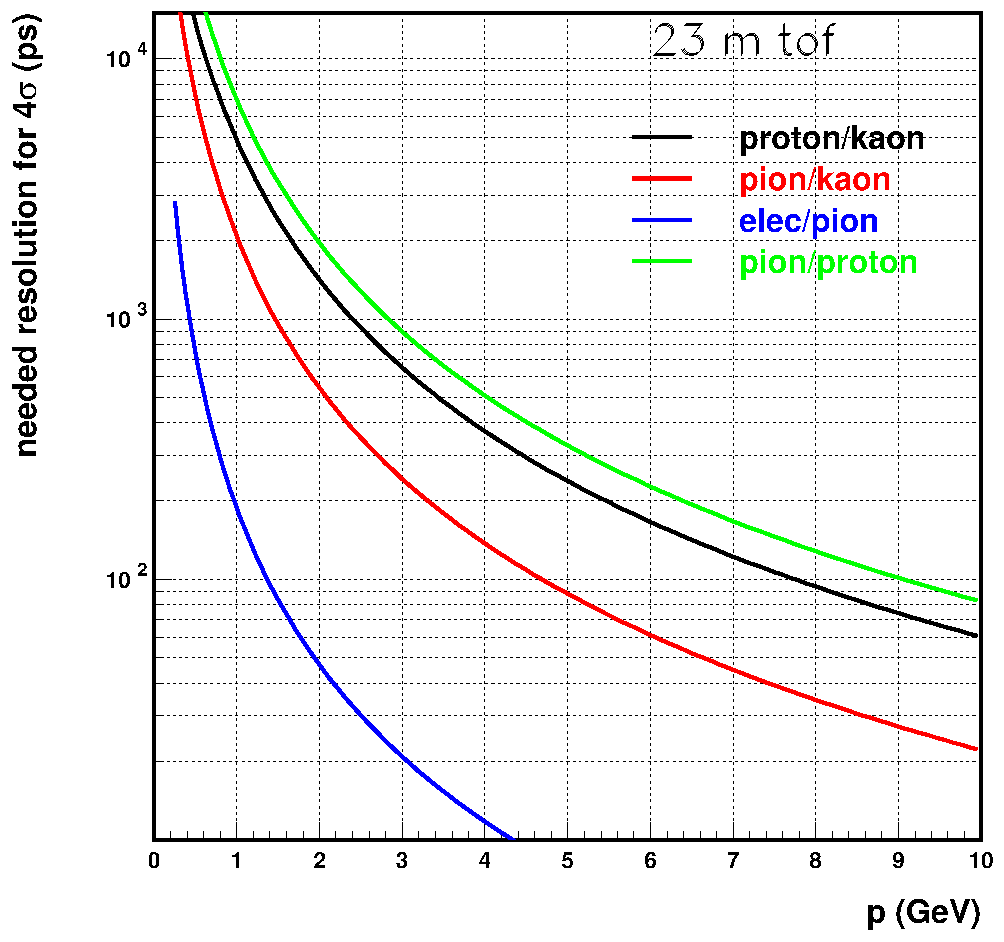
\includegraphics[width=0.85\textwidth]{toftaulow.pdf}
\end{cdrfigure}
\fixme{Enlarge axis labels and tick marks so that figure can be reduced in size and still be legible.}

\paragraph{LAPPD Time-of-flight system}
FermiLab is testing a ToF system that would utilize a 6 x 6 cm$^2$
large-area picosecond photodetectors (LAPPDs) (see figure \ref{fig:LAPPD}).
 The MCP-based devices
are capable of $< 50$~ps resolution with gains of $10^6-10^7$,
mm-position resolution along one axis and slightly worse resolution
along the other axis.  The photodetector is mounted on a readout
board, so the relevant exterior dimensions are 165.1mm x 109.3mm and a
thickness of 16mm. The active area is defined by the 4 squares visible in figure \ref{fig:LAPPD}, and amounts to about 8~cm$^2$.
\begin{cdrfigure}[LAPPD]{LAPPD}{Photo of one LAPPD device as proposed for the H2 and H4 beamlines.}
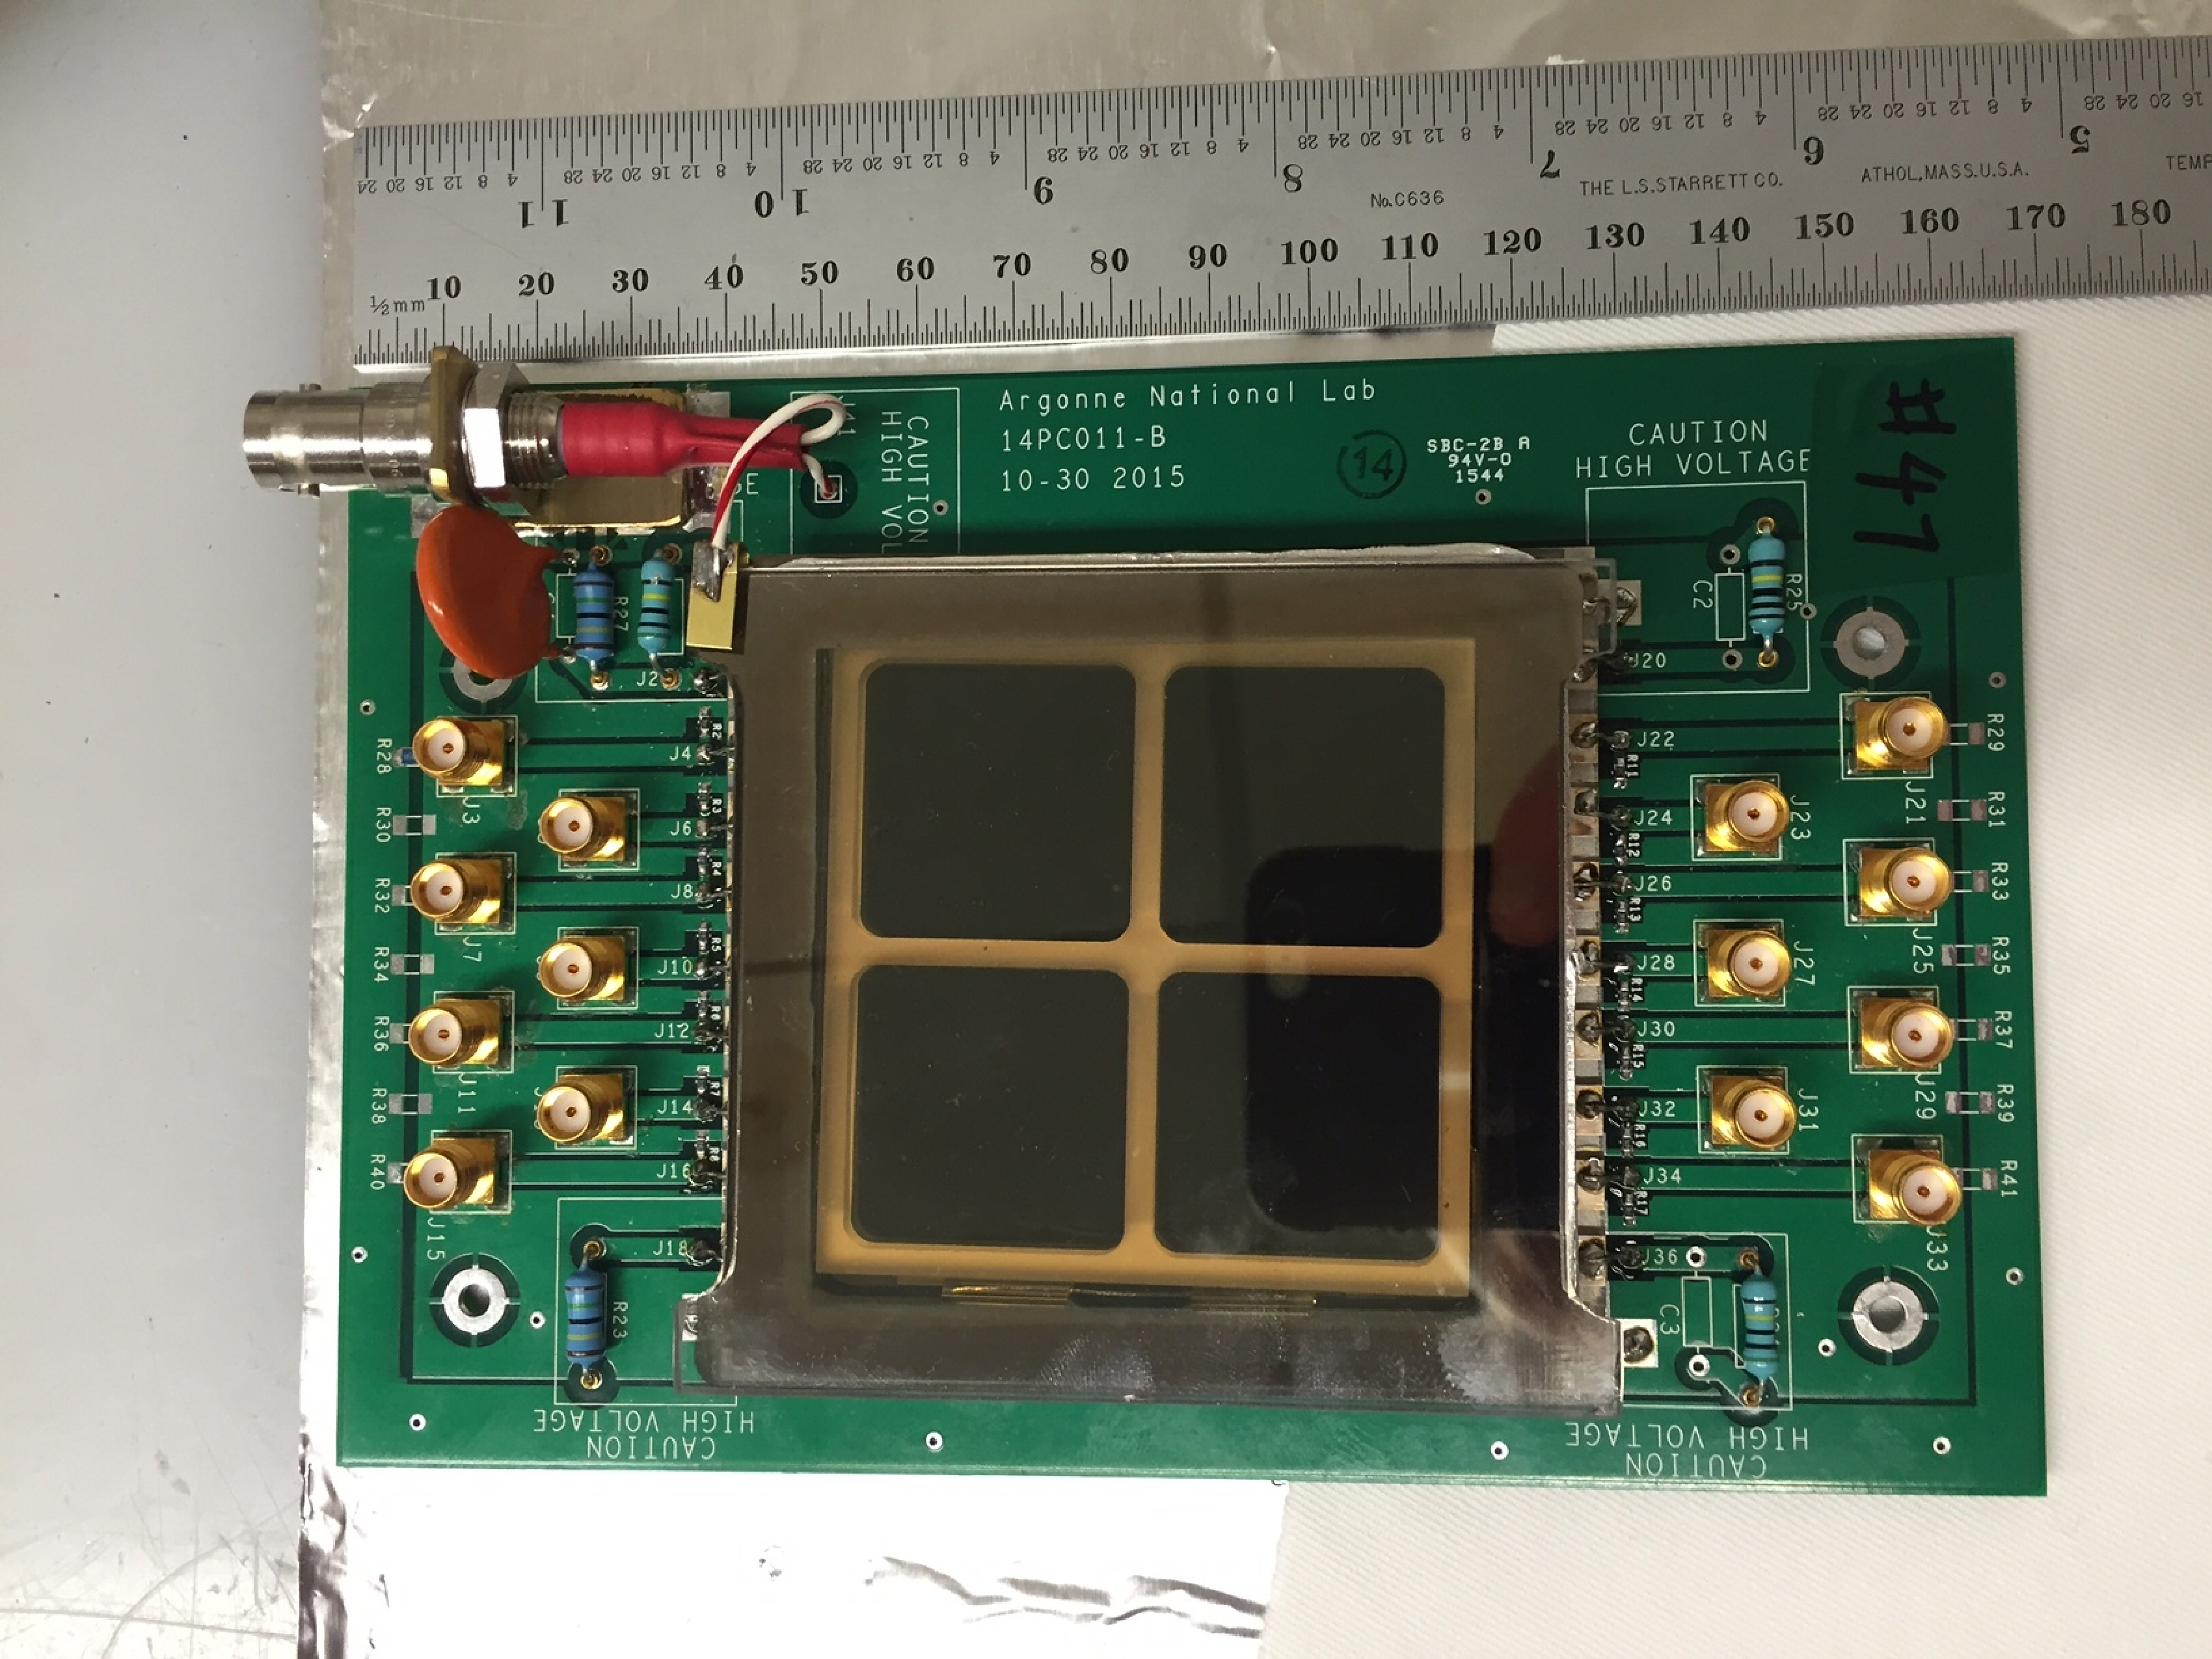
\includegraphics[width=0.65\textwidth]{LAPPD.pdf}
\end{cdrfigure}

\paragraph{Other Time-of-flight system}
Investigations are ongoing on the possibility of using the  scintillating fiber monitors for ToF purposes with the goal of a 1~ns timing resolution. The idea is to readout the detectors with the STiC ASIC \fixme{need reference} for SiPM readout.
%%%, developed at the  Kirchhoff Institute for Physics in Heidelberg - will be clear from reference
In this configuration, the time resolution would be dominated by the fiber response. A small prototype will be built and tested.

\fixme{Overall the beam line instrumentation section could benefit from a more clearly stated plan. The reader is left to guess what will and will not be built.}

\subsection{Material Budget and discussion}
Summing up all the required instrumentaton, the ``full'' beam line should include
\fixme{should include OR will include ?? see earlier comments about 2nd Cherenkov counter. TOF counters ...}
 5 beam monitors (2 for tracking and 3 for spectrometry), two ToF devices, two 2~m long Cherenkovs at high density or pressure. The material budget would be much too high for operation at low momenta
 \fixme{quantify what "low" means}
 , and in general for operation with electron beams.  
A full FLUKA \fixme{need reference} simulation of materials in the beamline and of the ProtoDUNE detector, including the beam window details, has been used to evaluate the effect of materials. 
\fixme{Should also mention that a second simulation was performed using GEANT 4 and that consistent results were obtained.}
Since the final layout of the beamline optics was delivered only recently, the simulations presented here assume a straight line with an initially parallel beam, deflected only by scattering. Particles are assumed to be ``lost'' when scattered outside of the beam pipe. Implementation of the magnetic elements is underway.
 Figure~\ref{fig:matblfull} shows the evolution of the material budget with a full instrumentation, assuming LAPPD for ToF. The total, including the beam window, would add to $0.6X_0$, 0.15 interaction lengths, and an energy loss for a mip of 28~MeV.
The largest energy loss contribution comes from Cherenkov detectors and from the  ToF system. Cherenkovs are useless for low energies (except a low-pressure one for electron discrimination) and can be easily removed from the beamline and substituted with a section of vacuum pipe.  
In a situation without Cherenkovs, the LAPPD devices plus monitors would still account for almost  $0.2X_0$. Besides energy degradation, scattering of low energy particles would  further degrade the pion and proton content of the beam.  Figure~\ref{1GeVtof} show examples of the beam degradation due to materials at 1~GeV/c: The rate of pions arriving at the detector is reduced by a factor 2.5, and the energy spread rises to 1.2\%. The rate of protons stopping in the detector is reduced by a factor 4, and the energy spread amounts to 2\% rms. This calculation is done in optimistic conditions, that is neglecting the efficiency loss due to the small active area of the LAPPD devices.

A possible way out would be the use of scintillating fibers as ToF devices for the lowest energy beams ($< 2 GeV$). 
\fixme{Has this been decided ? What is the plan ??}
 The feasibility of a fully plug-and-play beamline, with detectors going in and out, including those that need vacuum segmentation, is under discussion. 
 \fixme{In TDR cannot say that it is under discussion; need a baseline solution and possibly an alternate solution.}
 It has also to be noted that a good performance of the (combined) ToF system could avoid the use of non-standard Cherenkov counters.
\fixme{What are "non-standard" Cherenkov counters ??}
 \begin{cdrfigure}[Material budget]{matblfull}{Material budget in the beam line, as a function of the distance from the center of the detector (in cm). The red line describes the amount of $X-0$, the black line the amount of interaction length, both read on the left axis. The black dotted line is the average energy lost by a mip particle, and is read on the right axis (in MeV). Vertical lines show the positions of the various beam monitors (in between the two blue lines are the 3 devices for spectrometry, ``bm'' is the last beam monitor, ``bw'' is the starting point of the beam window).}  
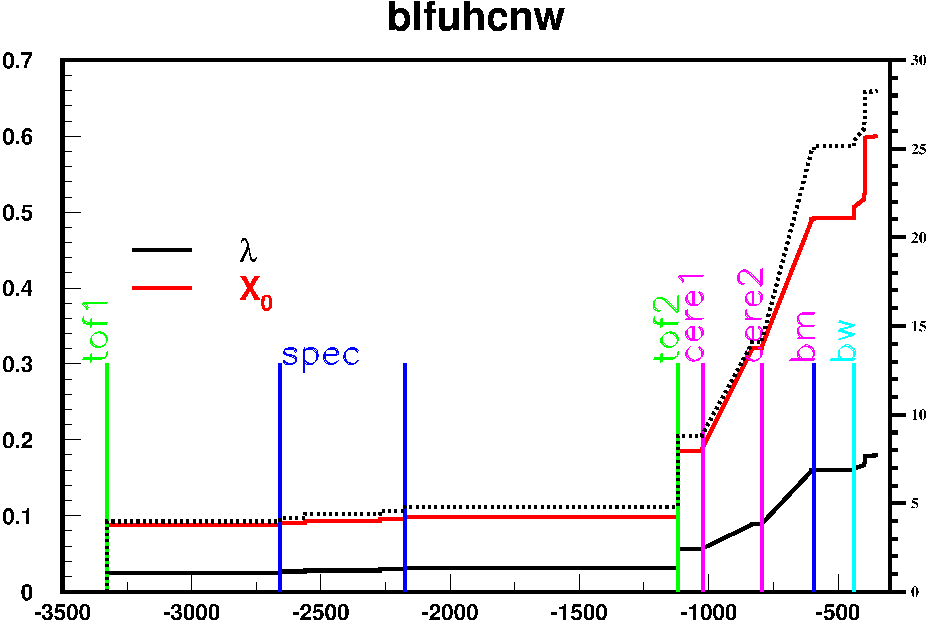
\includegraphics[width=0.65\textwidth]{blfuhcnwrayplo.pdf}
\end{cdrfigure}
\fixme{remove funny title of plot; add axes labels}
%
 \begin{cdrfigure}[Effect of materials at  1GeV]{1GeVtof}{Effect of materials at  1GeV/c. Left: $\pi$ beam, energy of the particle entering in the detector, in three conditions: with  beam monitors, with beam monitors and LAPPD for ToF, with the whole beamline filled with air (and no instrumentation). Right: proton beam, energy deposited by protons stopping in the LAr active volume, in three conditions: without instrumentation (the beam window is always present), with the scintillators only, and with scintillators plus LAPPD for ToF.  }
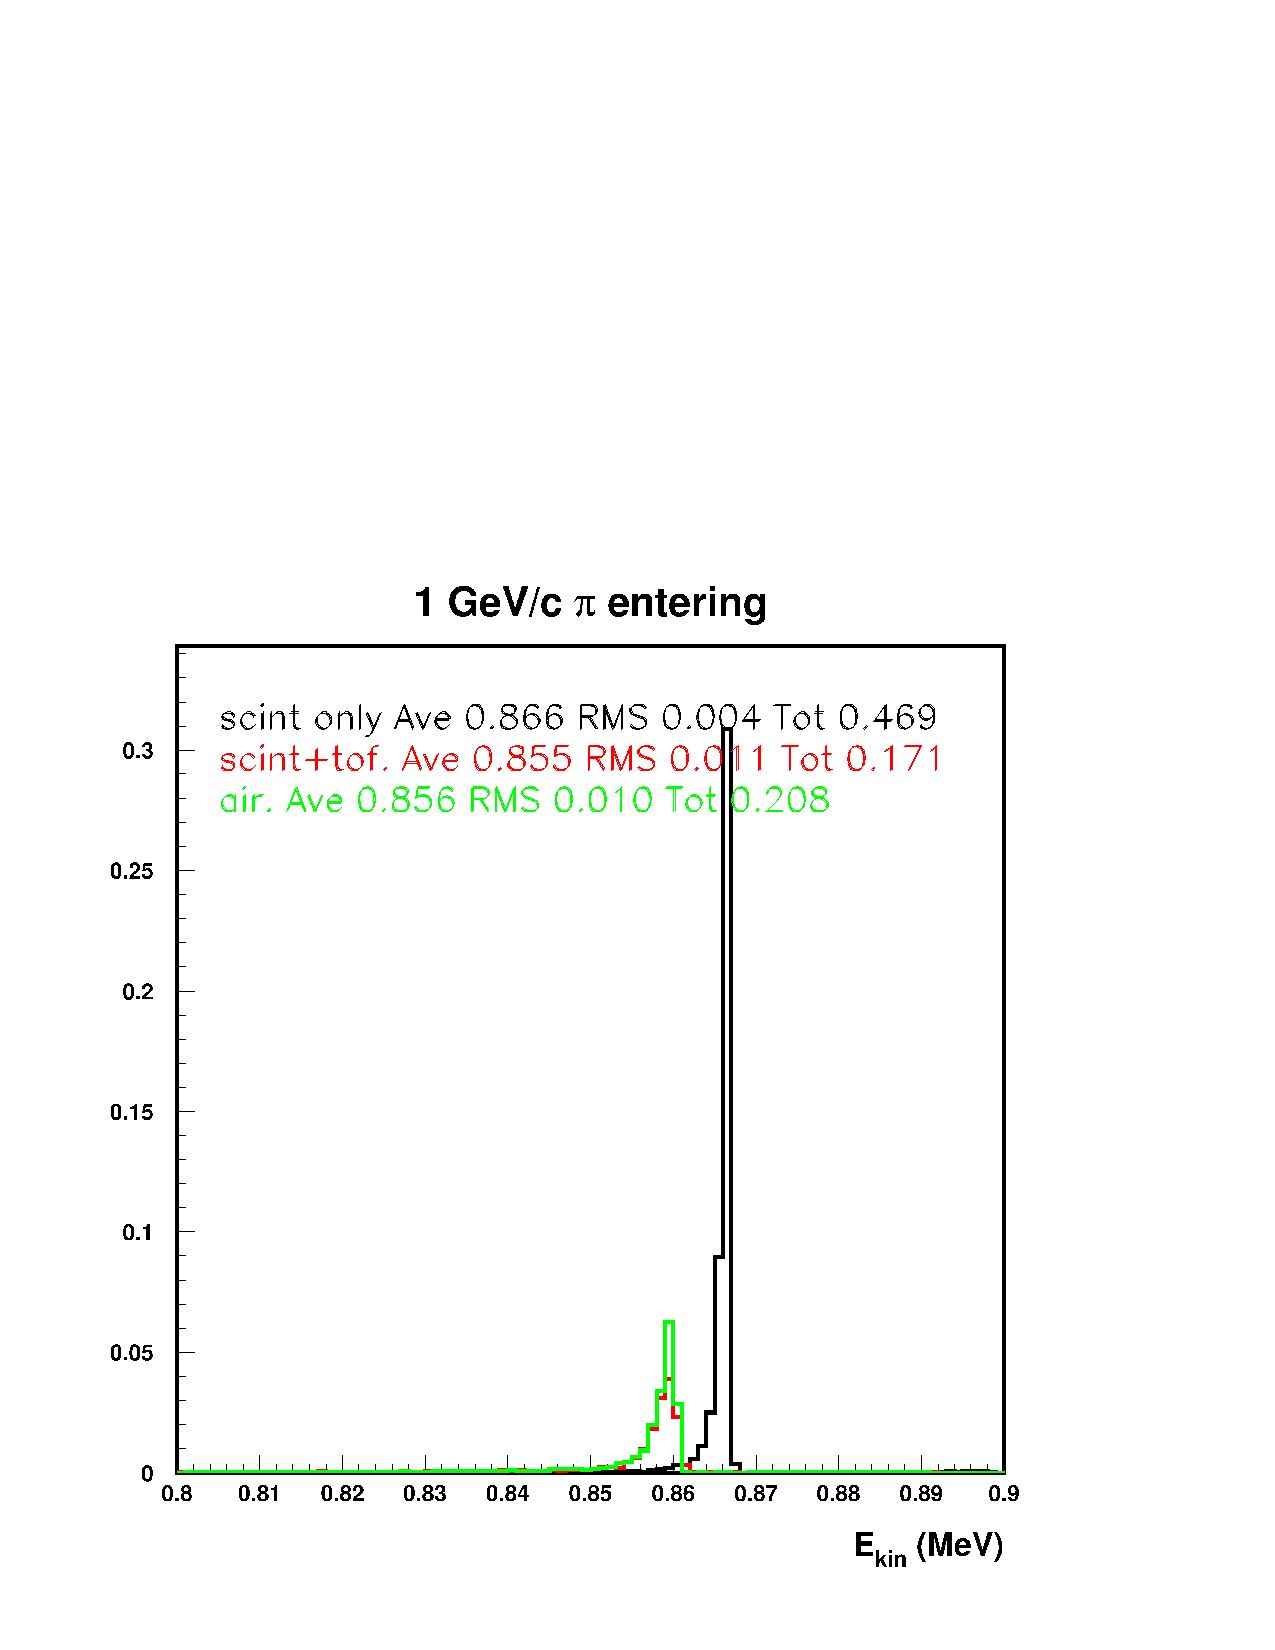
\includegraphics[width=0.45\textwidth]{pi1p0gev_innw.pdf}
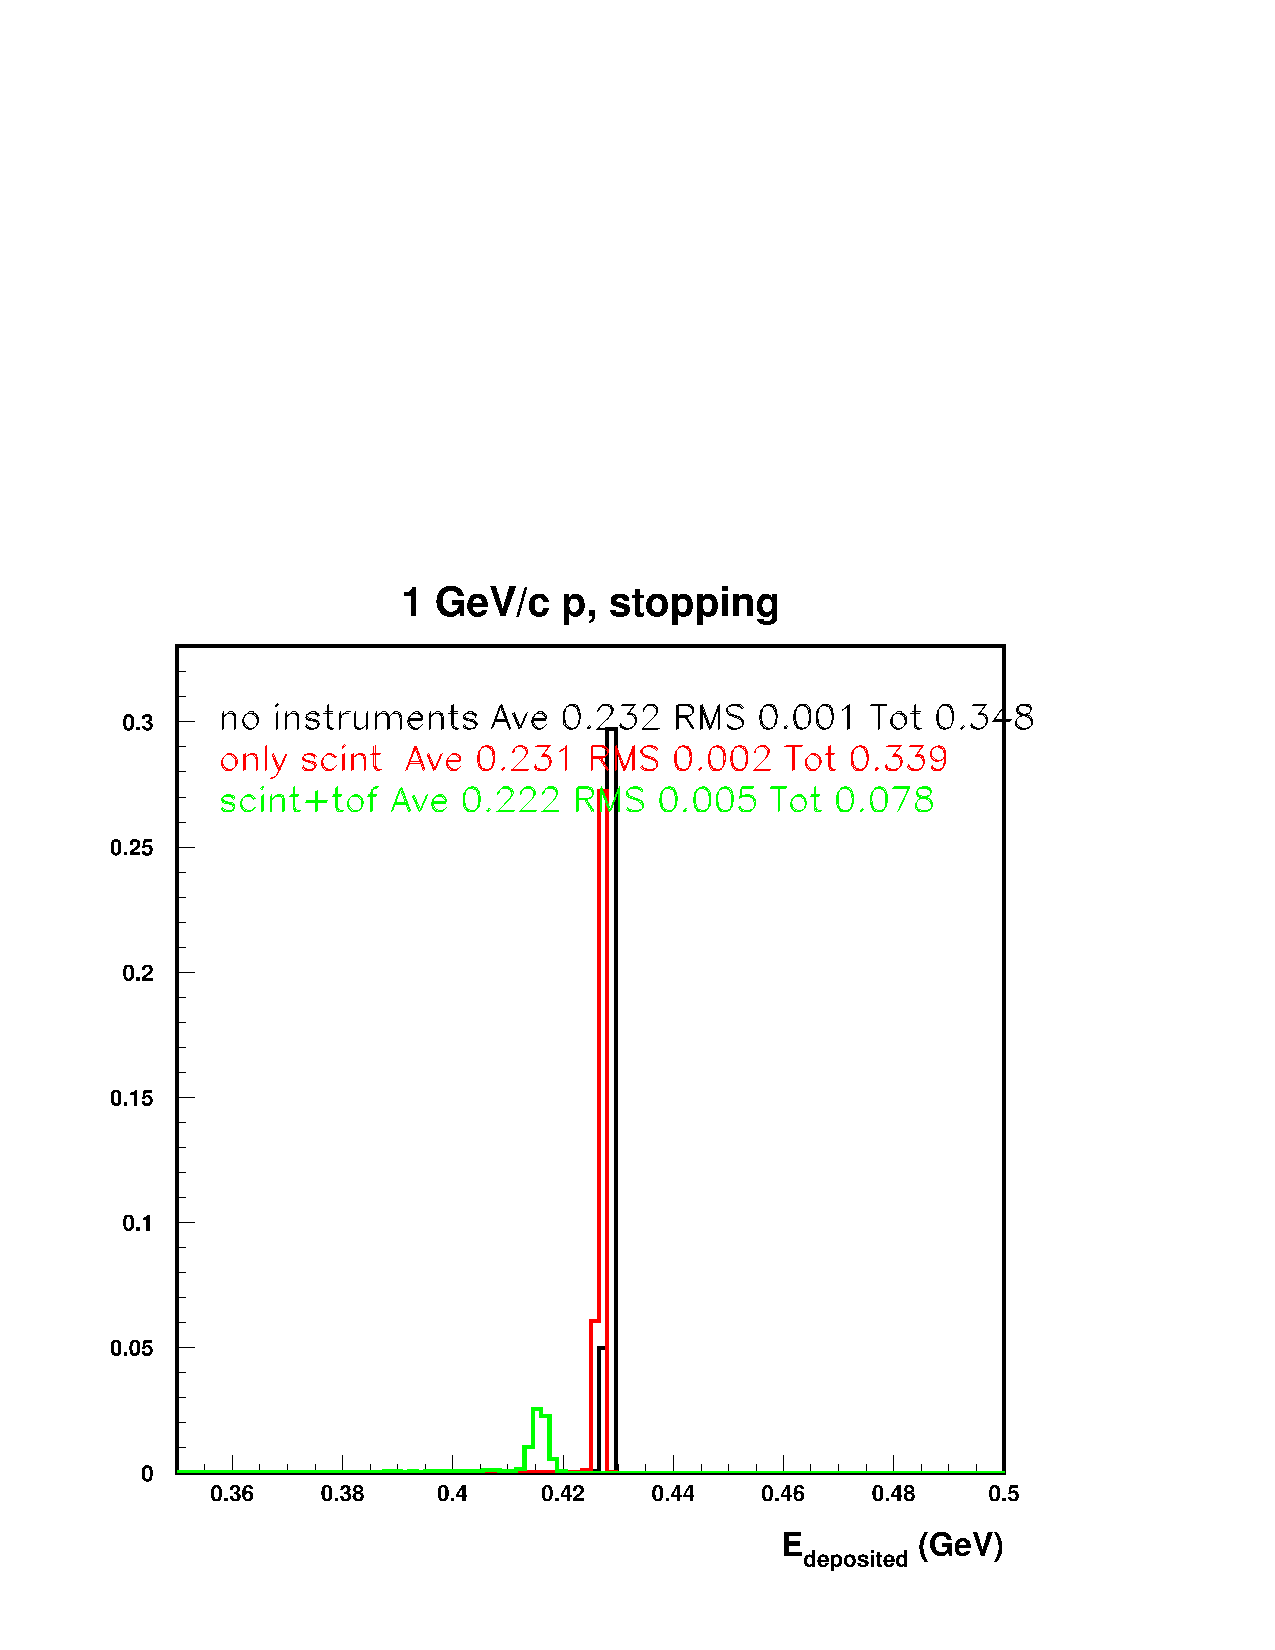
\includegraphics[width=0.45\textwidth]{p1gevstopnoqnw.pdf}
\end{cdrfigure}
\fixme{Fig. 7.11 does not seem to have reference in text.}

\subsection {Trigger and data acquisition}
Discussions are ongoing 
\fixme{Once more: cannot say that discussions are ongoing ...}
on how to provide a trigger signal from the beam instrumentation, and how to merge the beam instrumentation data into the TPC event. Synchronization will be ensured by a common time stamp through a White Rabbit network.
\fixme{Has white rabbit been agreed on ?}
 White Rabbit is a fully deterministic Ethernet-based network for general purpose data transfer and synchronization. It can synchronize over 1000 nodes with sub-ns accuracy over fiber lengths of up to 10 km. It is developed and widely used at CERN.
